\documentclass{article}
\usepackage{amsfonts}

\title{WhyWhere: An R  Package for Fuzzy Spatial Modelling}
\author{David Stockwell \hspace{0.4cm} }
\date{}

\usepackage{Sweave}
\begin{document}
\Sconcordance{concordance:article.tex:article.Rnw:%
1 11 1 1 0 34 1 1 2 1 0 1 2 1 0 5 1 3 0 1 2 25 1 1 2 4 0 1 2 104 1}



\maketitle

\begin{abstract}
This introduction to the R package WhyWhere is a rewritten
version of  Stockwell,  which
describes the mathematical basis and the operation of the package. The package extends other useful packages like raster and dismo with methods to fit, plot and test conjunection of fuzzy membership functions although more complex logical expressions are planned.  We show the model is simple and intuitive, efficient to compute, and at least equal to the best alternative approaches.  Thus, it makes a powerful tool to display information about species and their environmental relationships and to assess their significance.
\end{abstract}

\section{Introduction} \label{sec:intro}

This package is concerned with the development of interpretable models of self-directed entities such as biological species, although the approach could potentially be used in the other fields such as consumer and military intelligence, linguistics and control systems.  The technical basis is fuzzy set theory, where instead statmenets that are either true or false, a membership function describes a fuzzy truth value as a function $f: \mathbb{R} \rightarrow to [0,1]$ from a variable $V$ to the real unit interval $[0,1]$.  One must consider membership functions taking values from other spaces such as categories, (also known as factors in R) $N$ or on a space of many variables $V_1 \times V_2 \times ... \times V_n$ where each $V_i$ is an interval in $N$ or $R$. 

Experience has shown that a particularly useful way of combining unitary membership functions to resemble the AND, OR and NOT operators of classical logic are Zadeh operators:

AND: $x \land y = min(f(x),f(y))$, \\
OR: $x \lor y = max(f(x),f(y))$, and \\
NOT: $ \lnot x = (1-f(x))$.  


There ave been many approaches to learning fuzzy rules from from given data, and approaches to representation of the discovered rules.  One of the outstanding problems is the trade-off between accuracy and interpretability, or prediction and explanation in the ecological literature.  In particular in this package, ecological theory can motivate our approach, thus satisfying both criteria.  It is the desire to address the problem of explanatory models that motivated t development of WhyWhere -- to describe Why is a species Where? -- without sacrificing predictive accuracy or computational tractability.  

The guide is arranged as follows.  Section 2 describes the main operations, data preparation, developing the membership functions, the operations for building more complex models, and evaluation.  Section 3 compares the performace with the current best methed MaxEnt on a couple of known datasets.

\section{Basic Functions}

\subsection{Data Preparation}

Data are generally obtained as coordinates.  But need in a table with the presence or absence first.  Data preparation from these geocoordinates and environmental variables can proceed  as per the package raster for the environmental variables.  This is usually in the fomr of a RasterStack class.

However, the WhyWhere package adds some functions.  One can prepare a set of rasters with different resolutions but the same crop extent to give a raster pile.  


\begin{Schunk}
\begin{Sinput}
> source("../R/ww1.R")
> library(maptools)
> library(dismo)
> data(wrld_simpl)
> file <- paste(system.file(package="dismo"), '/ex/bradypus.csv',sep='')
> bradypus <- read.table(file, header=TRUE,sep=",")
> files <- list.files(path=paste(system.file(package="dismo"), 
+     '/ex',sep=''), pattern='grd', full.names=TRUE )
\end{Sinput}
\end{Schunk}

With this we prepare a data as file names.  

Next we are given a species presence, or presence and absence data, this function removes duplicates, and extracts environmental values from the pile, and appends a set of randomly selected points if necessary.

\begin{Schunk}
\begin{Sinput}
> Pres=bradypus[,-1]
> ext1=c(range(Pres[,1]),range(Pres[,2]))
> ext=ext1+c(-0.5,0.5,-0.5,0.5)
> Back=cbind(lon=runif(100,ext[1],ext[2]),lat=runif(100,ext[3],ext[4]))
\end{Sinput}
\end{Schunk}

The data to represent is an array with the first column is the presence absence and the other variables are the environmental variables at that location.  We will shortly have cloud based data access.  

\subsection{Membership Function}

In ecological niche theory a species tends to be more abundant, or be more likely,  within a range of an environmental variable.  The typical variables used are temperature  and precipitation ranges, although categorical variables such as soil and vegetation type, habitat structure are usually possible.  

The locations where the species occurs can be thought of as a sampling of the environmental space.  That is, while the counts of the environmental values has a distribution $E_i$ for $i$ over the range of the variable, the distribution of the sample where the species is present is $S_i$ over the samevalues $i$.  The most significant variable has the greates difference between these distributions.  The membership function is developed from the ration of counts   $S_i/E_i$. 


\begin{figure}[htbp]
\begin{center}
\begin{Schunk}
\begin{Sinput}
> #This one gives best variable var1
> models=lapply(files,function(x) membership(x,Pres,Back,extent=ext))
> plot.membership(models)
\end{Sinput}
\begin{Soutput}
[[1]]
NULL

[[2]]
NULL

[[3]]
NULL

[[4]]
NULL

[[5]]
NULL

[[6]]
NULL

[[7]]
NULL

[[8]]
NULL

[[9]]
NULL
\end{Soutput}
\end{Schunk}
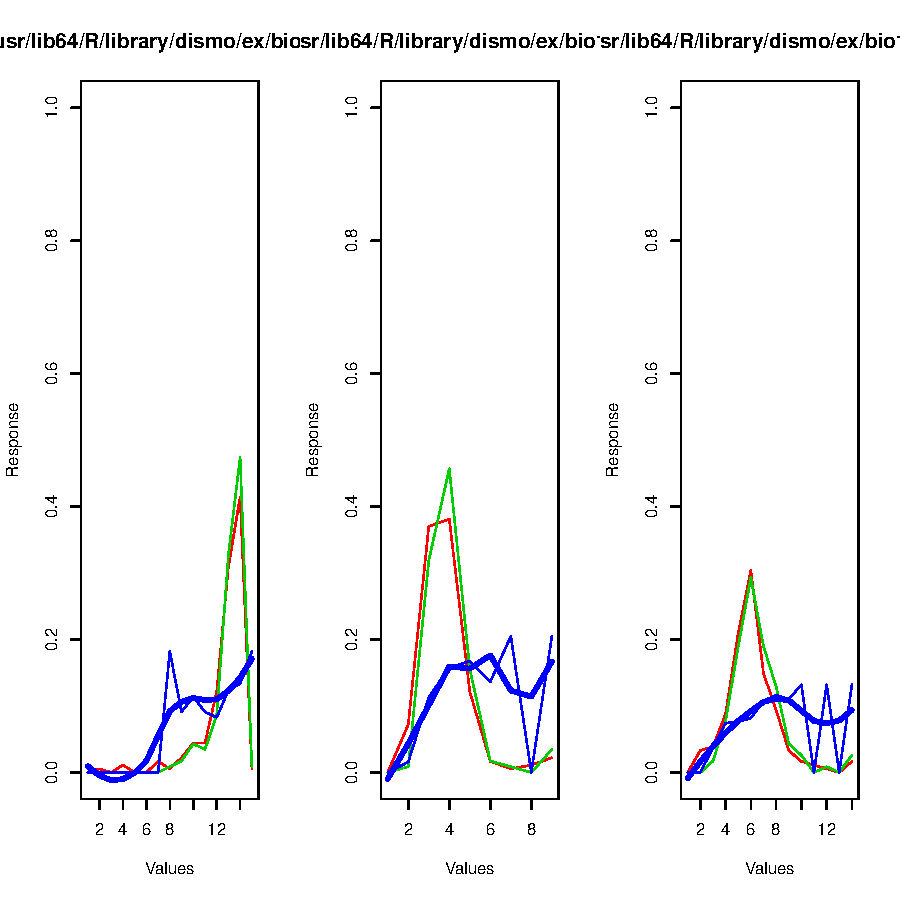
\includegraphics{article-003}
\caption{\label{fig:ts} Bradypus data set with response function plotted.}
\end{center}
\end{figure} 


While the classic approach to evaluating the significance is the Chi-squared test, we bin the samples of the environment and the location on the same ranges of values.  In the case of continuous variables there are chosen by R.  In the case of factor variable the categories remain as given. 

However Chi2 doesnt work in evaluating the multivariate case.  To evaluate both unitvariate and multivariate combination of environmental variables, we predict the probability of presence on each location and calculate the area under the curve of the reciever operating statistic (AUC for short).  

There is a further statistic that is the area under rank correlation or AUC. This arises where a models outputs a figure in the range of zero to one, but a prediction must be made in of 0 or 1. We must select a cuttoff value for the prediction to assign to zero or one.  The AUC is the probability that would give use the optimal accuracy.

A high AUC indicates that sites with high membership are more likely to be areas of presence, and vice versa.  An AUC score of 0.5 is no better than random.  The AUC can be calcualted from.

mean(sample(f(P==1),1000,replace=T)>sample(f(P==0),1000,replace=T),na.rm=T)


One may also consider other derivations of the membership function that resemble more closely the probability in Bayesian updating, can be viewed as a relaxation of some aspects of strict Bayesian statistics, that has proven simple and useful where strict Bayes.  

$P(S|E)=P(E|S)P(S)/P(E)$

But the problem is these rations of counts are not strictly probabilities.  In any sense, probability of the occurrence of a species P(S) is not well defined, or not generally of interest.  In typical example the probably of finding a species is dependent on season, search effort, and so is not well controlled.  Usually we only want to know the best areas to search for a species, as predicted by the most signifiant environkental variables.  So dropping the P(S) we still have a proportional relationship which sufficient to compare alternative environmental variables.  

$P(S|E)\propto P(E|S)/P(E)$ 

Other similar developments are using in MaxEnt where the membership is done using more complicated.  The results are very similar as the final comparative section shows.

\subsection{Fuzzy Conjunctions}

In the one dimensional case the variable with the largest significance is the best to select.  This gives a list of variables that the species responds to the strongest.  

But when we add more responses into a fuzzy expressions in a multi-variable datasets the most accurate conjunctive expression may not contain the best single variable.  This means we cannot use such methods as greedy search to identify higher dimensional expressions.  

The problem of expressing environmental relationships of more than one variable has been an important topic in statistical and ecological research, generalized linear modelling {} machine learning {} on the other.  Here we need to consider the logical relationship between variables that are expected from ecological theory.


\subsubsection{Law of the Minimum}

The principle of Liebig's Law of the Minimum states that growth is controlled by the scarcest necessary resource.  This is logically an AND operation or a fuzzy conjunction of limiting factors.  Note that a model composed of an arithmetic sum would represent the concept of growth determined by the overall sum of resources contributed from different sources, and so is not consistent with the Law of the Minimum.  Most model used to predict species distributions are of this form, and so their capacity to explain species distributions is questionable. 

\begin{Schunk}
\begin{Sinput}
> data=sapply(models,function(x) x$data$prob)
> cause=expression(models[[1]]$data$pa,data,dimensions=2)
> head(cause)
\end{Sinput}
\begin{Soutput}
      4.6       2.7       2.8       3.6       4.7       3.9 
0.5937500 0.5892857 0.5856287 0.5804111 0.5798611 0.5781434 
\end{Soutput}
\end{Schunk}


\subsubsection{Compeditive exclusion principle}

In ecology, Gause's law of compeditive exclusion is a proposition that two species competing for the same resource cannot coexist at constant populations if all other things remain equal, due to effect of slight advantages magnified over generations.  This behavioural shift leads to ecological niches.  This is logically an OR operation or a fuzzy disunction:

A possible example of this case is where a set of location actually contains two different species with different different habitats.  A disjunction of two habitats may model this case better.

\begin{Schunk}
\begin{Sinput}
> data=sapply(models,function(x) x$data$prob)
> cause=expression(models[[1]]$data$pa,data,dimensions=2)
> head(cause)
\end{Sinput}
\begin{Soutput}
      3.9       6.7       2.9       4.5       2.7       6.9 
0.5983112 0.5933661 0.5933413 0.5813107 0.5787589 0.5780142 
\end{Soutput}
\end{Schunk}


\section{Comparison - Bradypus and MaxEnt}

We test other models against the response output for the single dimensional case.  The response functions for MaxEnt and WhyWhere are quite similar as follows.



The following are the AUC results for MaxEnt and for WhyWhere in the one, two and 3 dimensional cases. The results of the model can be plotted using the rasterize package.

\begin{figure}[htbp]
\begin{center}
\begin{Schunk}
\begin{Sinput}
> nos=as.numeric(strsplit(names(cause)[1],"[.]")[[1]])
> newfiles=files[nos]
> Bmodels=models[nos]
> result=predict.membership(newfiles,Bmodels,extent=ext)
> par(mfcol=c(1,1))
> plot(result)
> points(Pres, col='blue')
\end{Sinput}
\end{Schunk}
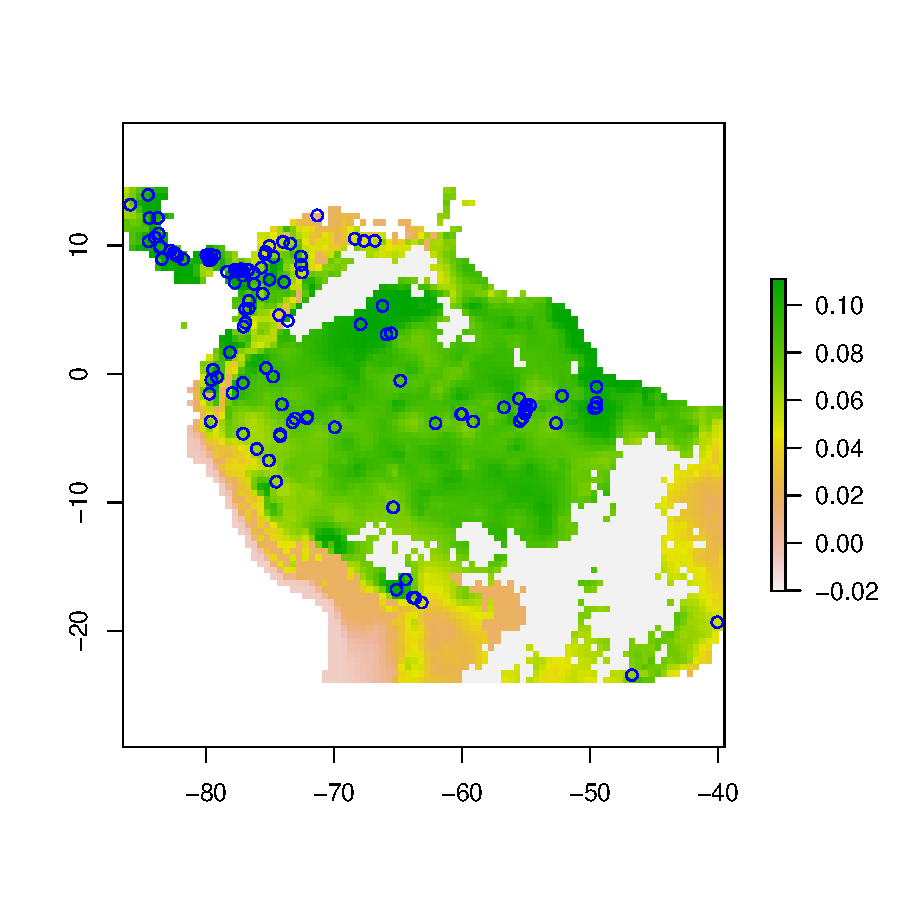
\includegraphics{article-006}
\caption{\label{fig:ts} Simulated random time series with SD=1 and level change of ith response plotted"}
\end{center}
\end{figure} 

\section{Conclusion and Further Work}

The R package WhyWhere is a useful packages to fit, plot and test empirical species as a conjunction of response functions.  More complex logical expressions are planned, as are improvements in computational efficiency and access to cloud data.  The method provides simple and intuitive, efficient to compute, and typical predictive results that are at least equal to the best alternative approaches.  



\bibliographystyle{ieeetr}
\bibliography{library}

\end{document}
